%-------------------------------------------------------------------------------
\chapter{Benchmark Composition}
\labelchapter{app.benchmark}

    In order to analyse how the defined methodologies can be leveraged to improve the life of hardware developers, we implemented {\bf 7 computation kernels} using \chisel, which are introduced in Table \ref{app.benchmark:table.benchmark}.

    Each kernel has been developed by applying the {\bf meta design methodology} introduced in section \ref{ch.dse:sec.definition:ssec.meta}, and this appendix also exposes --- in addition to the benchmark description --- which considerations were taken into account, for each kernel, in order to provide an explorable meta design from a prior algorithmic analysis. 

    This benchmark is proposed as an open-source project \cite{ferres_benchmark_2021}.

    \section*{Kernel model}
        The kernels were built to be integrated in a simple programming model, by exposing a unified interface.
        To do so, we defined a \chisel{} {\bf Role} and {\bf Shell} based architecture, as can be seen in emerging \myLongAc{FPGA}{Field-Programmable Gate Array} projects that aim at separating the accelerators implementation from their interfaces \cite{caulfield_cloud-scale_2016}.

        The proposed interface is kept simple, as {\bf Role} simply exposes a bi-directional {\bf Ready/Valid} interface with a parametric {\it bandwidth} (Fig. \ref{app.benchmark:sec.kernel:fig.model}), that can be then be integrated in more or less complex {\bf Shells}, ranging from simple mapping of this \myLongAc{IO}{Input/Output} to the communication \myLongAc{IP}{Intellectual Property} that may be available on the target board, to complex communication protocols.

        However, such structure is quite simple, and evolutions should consider integrating multi-lane communications for configuration purposes --- which are currently done using the same \myAc{IO} bus, meaning that the accelerators must consider configuration in their data communication protocols.

    \clearpage
        \begin{figure}[ht!]
            \centering
            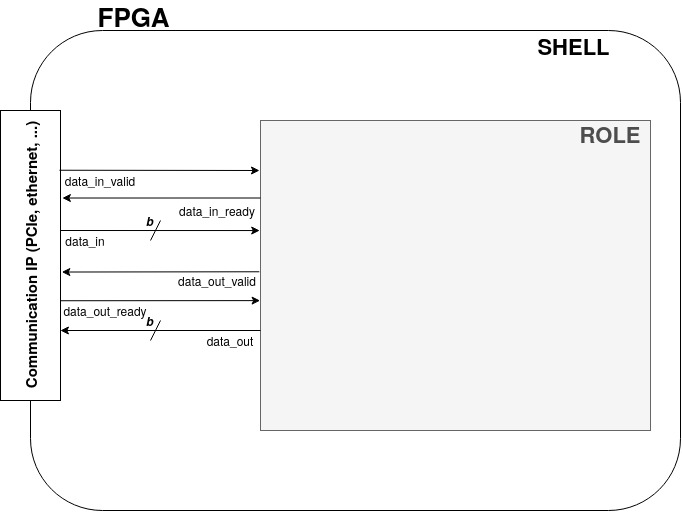
\includegraphics[width=0.9\textwidth]{Figures/shell.png}
            \caption{Simple Role and Shell model used}
            \label{app.benchmark:sec.kernel:fig.model}
        \end{figure}
        \vspace{-1cm}

    \section*{Dot Product}
        The dot product generator has been developed as a simple example, and does not expose a heavy design space.
        Moreover, an example of the target architecture is introduced in Figure \ref{app.chisel:fig.dot}.

        Given two vectors $a$ and $b$ of dimension $n$, we compute:
        \begin{equation}
            \label{app.benchmark:sec.dp:eq.formula}
            c = \sum_{i=0}^{n-1}a_i*b_i
        \end{equation}

        
        The {\it Vector width} is used to define the algorithmic complexity of the implementation, while both {\it dynamic} and {\it precision} define the element type to operate on.
        In order to take advantage of an \myAc{FPGA} implementation, we aim at exploiting the parallelism of the algorithm, while keeping the resource usage under given constraints.
        The dot product can easily be expressed in a functional way, using the {\bf Map-Reduce} pattern, implying we can extract a maximum parallelism level of $n$, by performing all the multiplications in parallel before performing reduction through additions.
        We thus expose {\it parallelism} as a parameter, allowing the user to easily increase the throughput at the cost of functional unit replication.

    \clearpage
    \section*{General Matrix Multiply}
\vspace{-0.2cm}
        The \myLongAc{GEMM}{General Matrix Multiply} algorithm is a generalization of the matrix multiply algorithm.

        Given three matrices $A$, $B$ and $C$ in $\mathcal{M}_n$, the set of the matrices of dimension $n \times n$ (that we consider square for simplification) and two values $\alpha$ and $\beta$, we compute:
        \begin{equation}
            \label{app.benchmark:sec.gemm:eq.formula}
            C = \alpha \cdot A \times B + \beta \cdot C
        \end{equation}
        A meta design for the \myAc{GEMM} algorithm has been introduced in prior work \cite{ferres2020chisel} --- from which Equation \ref{app.benchmark:sec.gemm:eq.throughput} is extracted --- and was manually explored in order to demonstrate how both {\bf meta design} and {\bf meta exploration} can be leveraged to increase designers productivity \cite{ferres_2021_integrating}.

        The \myAc{GEMM} generator has been developed in order to maximize the \myAc{IO} usage, targeting a temporal behaviour as represented in Figure \ref{app.benchmark:fig.gemm-chrono}.
        Such prior analysis enables to build a generic generator that uses both \myLongAc{BRAM}{Block Random-Access Memory} and \myLongAc{MAC}{Multiply and Accumulate} to build adaptable designs that will compute partial results on the fly, resulting in a theoretical maximal usage of the bus.

        \begin{figure}[h!]
            \center
            \scalebox{.8}{
                \begin{wave}{5}{14}
                    \nextwave{ready} \bit{1}{14} \bit{0}{1}
                    \nextwave{input} \known{$\alpha$}{1} \known{$\beta$}{1} \known{$C$}{4} \known{$B^t$}{4} \known{$A$}{4} \bit{0.5}{1}
                    \nextwave{valid} \bit{0}{11} \bit{1}{4}
                    \nextwave{output} \unknown[XXX]{11} \known{$result$}{4}
                    \nextwave{} \duration{$\Delta_c$}{15}
                \end{wave}
            }

            \caption{Targeted chronogram for an efficient GEMM implementation}
            \label{app.benchmark:fig.gemm-chrono}
        \end{figure}
\vspace{-0.3cm}
        Equation \ref{app.benchmark:sec.gemm:eq.throughput} introduces the theoretical throughput (in $operation\cdot second^{-1}$) of the designs generated from this description, and is used to define a cost function to be maximized while exploring the \myAc{GEMM} design space.
        One can remark that doing this enable to normalize a cost metric through different matrices dimensions, as performing {\bf one \myAc{GEMM} computation} over $\mathcal{M}_n$ is comparable to performing {\bf eight $\mathcal{M}_{\frac{n}{2}}$ computations}.

        \begin{equation}
            \label{app.benchmark:sec.gemm:eq.throughput}
            T_{GOp/s} = \frac{f}{\Delta_{cycle}} = \frac{2 \times n^3 \times f \times b}{3 \times n^2 \times e}
        \end{equation}

        As a result, we define three parameters for \myAc{GEMM} generation: the {\it bus bandwidth}, which defines the capacity of the \myAc{IO} bus, the {\it element bit width}, which defines the size of each element in the considered matrices --- meaning that $\frac{bandwidth}{bitwidth}$ element can be sent and received each cycle --- and finally the {\it dimension} (or $n$) of the matrices in $\mathcal{M}_n$.

    \clearpage
    \section*{Fast Fourier Transform}
        The \myLongAc{FFT}{Fast Fourier Transform} algorithm is used in signal processing to provide frequency analyses from temporal data.

        Given $x_0, ..., x_{n-1} \in \mathbb{C}$, \myAc{FFT} is computed using the following formula:
        \begin{equation}
            \label{app.benchmark:sec.fft:eq.formula}
            f_j = \sum_{k=0}^{n-1}x_k e^{-\frac{2\pi i}{n}jk}
        \end{equation}

        The \myAc{FFT} generator was built to maximize the \myAc{IO} bus usage, resulting in a pipelined implementation inspired from Gerez \cite{gerez_fft_2012}.

        The pipeline is based on the \myLongAc{R2MDC}{Radix-2 Multi-Path Delay Commutator} technique \cite{rabiner1975theory}, using multiple Radix-2 stages to reduce the \myAc{FFT} problem size by 2 at each stage, in a {\it divide and conquer} fashion.
        We use the \myLongAc{DIF}{Decimation In Frequency} mode in order to consume input data (temporal samples) in a \myAc{FIFO} fashion, resulting in a need to reorder the output data (frequency samples) at the end of the pipeline.
        This is done by using a {\bf Ping Pong buffer}, which enables to provide the frequency data in a coherent order, even if the \myAc{DIF}-based implementations produce out-of-order frequency samples --- moreover, using another {\bf Ping Pong buffer} on the \myAc{R2MDC} inputs enables to exploit them at 100\%.
        The {\bf Twiddle factors} --- \ie the trigonometric coefficients --- are computed {\it a priori} and stored in \myLongAc{ROM}{Read-Only Memories} to fasten the computations.

        This pipelined implementation allows to maximize the \myAc{IO} bus usage as we consume input data on the fly, while maximizing the resource usage.

        The \myAc{FFT} generator relies on three parameters: the {\it parallelism} level, which defines the number of lanes used in the \myAc{R2MDC} model --- \ie the number of inputs that can be absorbed in one cycle in the generated accelerator --- the {\it element bit width}, which defines the size of each complex element used for computation, and the {\it size} of the \myAc{FFT} problem being solved.
        As for the {\it element bit width}, the \myAc{FFT} uses {\bf Fixed Point} representation for the computations, and one could want to explore this representation by defining both {\it dynamic} and {\it precision} parameters. 
        However, as we do not focus \myLongAc{QoS}{Quality of Service} based exploration on this kernel, we chose to define the data representation using only one parameter --- we use $\frac{bit width}{2}$ as values for both {\it dynamic} and {\it precision}.

        We can remark that, in contrast with the \myAc{GEMM} implementations, two \myAc{FFT} implementations of different sizes cannot be compared easily, as the first one cannot be expressed by composing instances of the second one.
        We here solve different applicative problems, hence the developers either need to specify which size to use, or to allow the exploration process to make this decision through applicative information (\eg \myAc{QoS}).

    \section*{Finite Impulse Response Filter}
        \myLongAc{FIR Filter}{Finite Impulse Response Filter} is a standard digital processing algorithm, based on the application of a finite number of coefficients to temporal samples in order to modify an input signal.

        % Given a set of coefficients $c_0, ..., c_{n-1}$ and time indexed samples $x_t, t\in [\![0; +\infty ]\!]$
        The filter response is computed using a discrete convolution between an input signal $x[t]$ and the function represented by $c_k, k\in [\![0, n-1]\!]$ coefficients:
        \begin{equation}
            \label{app.benchmark:sec.fir:eq.formula}
            f(t) = \sum_{k = 0}^{n-1} c_k \times x[t - k]
        \end{equation}

        Once again, we aim at exploiting the \myAc{IO} bus at its maximal capacity by absorbing the whole input bandwidth as temporal samples at each cycle.
        To do so, a structured buffer is built to enable windowed accesses to the buffer data: if we consider that $k$ elements are presented on the input bus at each cycle, then those $k$ elements $e_i, i \in [\![0, k-1]\!]$ are fed to a \myAc{FIFO}. 
        On read, this structure enables to access $k$ different vectors for inputs ($[\![e_{i}, e_{i+k-1}]\!], i \in [\![0, k-1]\!]$), meaning that we can compute $k$ successive response of the filter $f(t+i), i\in[\![0, k]\!]$ in parallel.
        Doing so, we hence built a parametrizable, fully pipelined \myAc{FIR Filter} generator that takes the best of the available \myAc{IO} capacities.

        So built \myAc{FIR Filter} generator uses three parameters: the {\it bus bandwidth}, which defines the capacity of the \myAc{IO} bus, the {\it element bit width}, which defines the data representation used in the computations, and the {\it tap number}, which defines the number of coefficients used in the filter.
        A fourth parameter allows to define whether coefficients are hard-coded --- \ie stored in \myAcs{ROM} --- or provided in the communication protocol. However, no exploration process should consider both kinds of implementations as they are not comparable and depend on both applicative needs and target constraints.

        Here again --- as for \myAc{FFT} implementations comparison through multiple sizes --- it is difficult to compare \myAc{FIR Filter} implementations if the {\it tap numbers} differ.
        However, one could define application specific metrics to allow such comparison, for example by defining applicative needs --- \eg the {\bf filter type} ({\it low-pass}, {\it band-pass}, ...) or {\bf cut-off frequency} --- and running empirical simulations to choose which implementation best fit one's need.
        
    \clearpage
    \section*{Monte Carlo}
        Both {\it Pi} and {\it Black Scholes} kernels are based on a parametric {\bf Monte Carlo} generator, for which the meta architecture is introduced in Figure \ref{app.benchmark:sec.monteCarlo:fig.kernel}.

        In order to provide random samples following normal distributions for the different cores --- which are generated using different seeds --- we use a parametric Tausworthe generator to feed pre-computed {\bf Box-Muller} \myAcs{ROM} \cite{box1958note}.
        Using so defined samples, each core performs the given computations, and the partial results are averaged to provide a statistical value for the result --- for example, we estimate the value of $\pi$ by checking if random points are inside a circle of radius one before computing the proportion of points that are within this disk.
        This can be used to determine the area of the disk, hence we can empirically approximate $\pi$.

        \begin{figure}[h!]
            \centering
            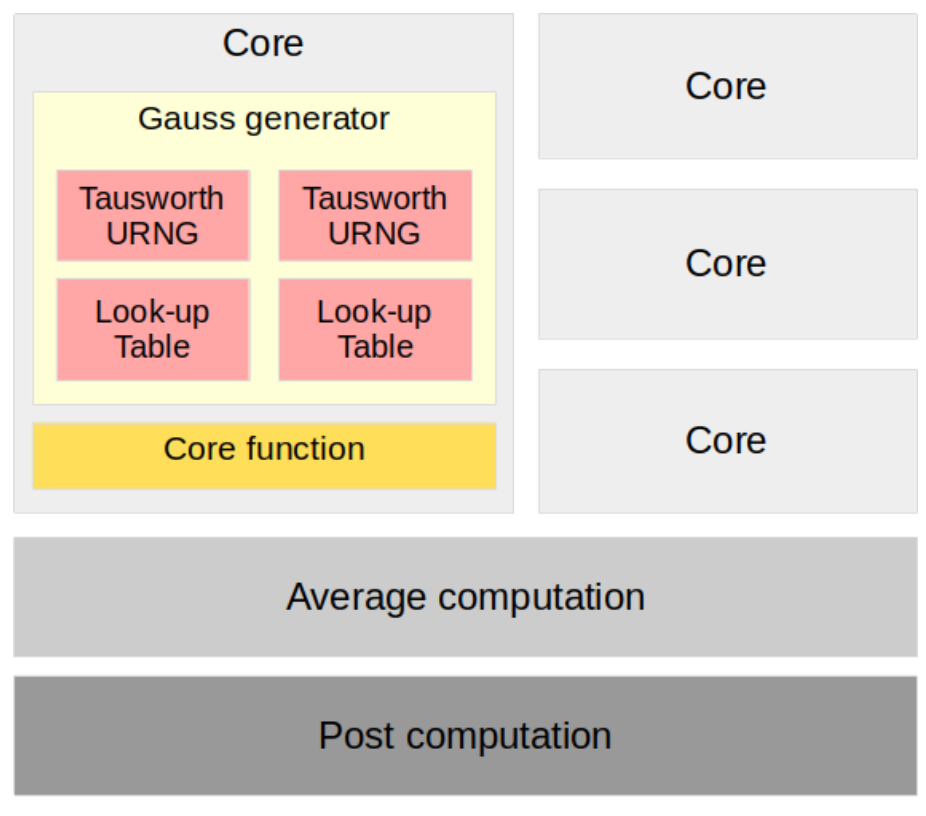
\includegraphics[width=.6\textwidth]{Figures/monteCarloCore.png}
            \caption{Monte Carlo kernel meta architecture}
            \label{app.benchmark:sec.monteCarlo:fig.kernel}
        \end{figure}

        We use a {\bf Factory pattern} to build different {\bf Monte Carlo} kernels, fully exploiting the \myLongAc{OOP}{Object-Oriented Programming} features of \chisel{} for such generators.
        This enables to build both {\it Pi} and {\it Black Scholes} kernels by defining specific inner functions while allowing code reusability by exploiting inheritance.

        For both kernel generators, we thus define four parameters: the {\it dynamic} and the {\it precision} to define the Fixed Point representation for the computations, the {\it iteration number}, which defines the number of experiments to be run before performing both average and post processing to provide a result, and the {\it core number} which defines the number of parallel cores to run iterations.

        As for the {\it Black Scholes} generator, we aim at computing the price of an action at time $t$, given the following equation --- $\mu$, $\sigma$ and $T$ being respectively the {\bf risk free rate}, the {\bf volatility} and the {\bf maturity} of the considered option:
        \begin{equation}
            \label{app.benchmark:sec.monteCarlo:eq.bs}
            S(t) = S(0)\times e^{(\mu - \frac{1}{2}\sigma^2)T + \sigma\sqrt{T}\mathcal{N}(0, 1)}
        \end{equation} 
        
        However, as  hardware-based computations of the exponential function are costly, we leverage {\bf Euler-Maruyama} method to sequentially approximate the formula (Eq. \ref{app.benchmark:sec.monteCarlo:eq.bs}):
        \begin{equation}
            \label{app.benchmark:sec.monteCarlo:eq.bsem}
            S_{\Delta t} = S_0((1 + (\mu - \frac{1}{2}\sigma^2)\Delta t) + \sigma\sqrt{\Delta t}\mathcal{N}(0, 1)
        \end{equation}

        To exploit this approximation model, the {\it Black Scholes} kernels are generated using a fifth parameter, namely the {\it Euler iteration number}, which is used to define how many iterations are taken for each {\bf Euler-Maruyama} based approximation.
        Moreover, other parameters could be considered for exploration, as this meta implementation uses hard coded values for the {\it Black Scholes} specific parameters ($\mu$, $\sigma$ and T), and for the {\bf Monte Carlo} parameters, such as the Tausworthe and the Box-Muller configurations.
        Such values may also be integrated in the communication protocol, in order to build dynamically programmable accelerators.

        For both {\bf Monte Carlo} based kernels, we hence expose heavy design spaces as the \myAc{QoS} is considered for exploration --- we aim at maximizing the design efficiency (\ie performance \vs cost ratio) while insuring that the generated designs does not generate significant errors with respect to a given workload model.

    \section*{Multilayer Perceptron}
        The \myLongAcs{MLP}{Multilayer Perceptron} are simple neural network models that are based on the original Perceptron model as introduced by F. Rosenblatt in 1958 \cite{rosenblatt1958perceptron}.
        They consist on a given number of {\bf fully connected} neuron layers --- meaning that each neuron of a layer $n$ is connected to every neuron of the layers $n - 1$ and $n + 1$.
        
        Such model has been used for more than twenty years for multiple uses, notably for image classification over the {\bf MNIST database} (handwritten digits) \cite{lecun_gradient-based_1998}.
        The \myAc{MLP} implementations are costly, as all the necessary connections result in a complex interconnection model, which led researchers to develop more compact neural network for \myLongAc{DL}{Deep Learning} --- especially for image processing and recognition domains --- such as \myLongAc{CNN}{Convolutional Neural Network} models.
        However, some specific domains still require to use fully connected networks --- \eg personalization and recommendation systems \cite{naumov2019deep} --- and given their simple structure, we chose to implement a \myAc{MLP} generator using \chisel.

        We chose not to base developed generator on the {\bf Role} model as introduced in Figure \ref{app.benchmark:sec.kernel:fig.model}, in order to allow a multi-channel interface model, notably to be able to configure the accelerator through a distinct \myAc{IO} bus.
        In order to take the best of \myAc{FPGA} specificities, we chose to target a {\bf fully unrolled} implementation, meaning that each neuron in the network will be an independent entity with its own memory and computation units --- in contrast to most hardware implementations which are based on scheduling the different neuron tasks on a topology-independent amount of hardware neurons --- as existing works proved that unrolling networks on \myAcs{FPGA} can lead to efficient implementations \cite{prost2017scalable}.

        Most of the design effort was done at {\bf neuron level}, in order to provide efficient basic units for computing neuron outputs.
        Let $N(i, j)$ be the $j^{th}$ neuron of the $i^{th}$ layer of a given network.
        $N(i, j)$ got $n$ different inputs $x_0, ..., x_{n-1}$ resulting from the preceding layer, $n$ different weights $w_0, ..., w_{n-1}$ that result from a prior training of the network and are used for configuration purposes, and a bias $b$ which is also provided by the training phase. 
        An {\bf activation function} $f$ is also applied to each neuron output, and is defined at network level --- thus it does not need to be configured at neuron level as it is defined at elaboration time and can be hard-coded.

        The output $o(i, j)$ is then computed using the following formula:
        \begin{equation}
            \label{app.benchmark:sec.mlp:eq.formula}
            o(i, j) = f(\sum_{k = 0}^{n-1} x_k w_k + b)
        \end{equation}

        A simplified version of the chosen neuron architecture is introduced in Figure \ref{app.benchmark:sec.mlp:fig.neuron}.
        Each neuron is composed of an embedded memory --- which should leverage \myAcs{BRAM} for \Xilinx{} boards --- to store network weights, and a computation unit to perform \myLongAc{MAC}{Multiply and Accumulate} operations.
        As \myAc{MAC} operations can easily be parallelized in a way similar to the dot product, we hence expose a {\it parallelism} parameter at neuron level to easily define the \myLongAc{FU}{Functional Unit} replication factor.
        In order to properly schedule the output propagation, a {\it scan-chain} system is inserted after the activation function, to manage the synchronization with the next layer.

        \begin{figure}[h!]
            \centering
            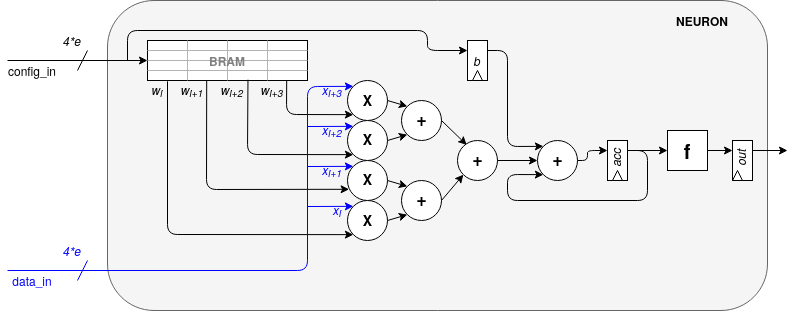
\includegraphics[width=1.0\textwidth]{Figures/neuron.png}
            \caption{Simplified schematic for a neuron implementation}
            \label{app.benchmark:sec.mlp:fig.neuron}
        \end{figure}

        Each neuron also includes a parallel data bus for configuration, which uses a simple \myLongAc{FSM}{Finite State Machine} to write weights in a \myAc{BRAM} --- weights are written in a vector-like structure, enabling to access to $k$ weights $w_0, ..., w_{k-1}$ each cycle, in order to feed $k$ \myAc{MAC} units in parallel.
        
        Using this basic neuron generator, we thus define the whole network as a composition of layers, each layer being defined as a composition of neurons, with small \myAcs{FSM} for the control flow --- including two different \myAc{IO} buses, respectively for the data and the weights.

        We chose to use MNIST as a use case for so defined \myAc{MLP}, as it is both a simple example and a standard reference in image processing.

        Beside the {\it parallelism} parameter, which allows to explore a trade-off between the neuron throughput and its resource usage, we defined three parameters: {\it \#neuron($1^{st}$ layer)} and {\it \#neuron($2^{nd}$)} respectively to define the number of neurons in $1^{st}$ and $2^{nd}$ layers, while the {\it element bit width} once again defines how data are represented in the design.
        We here only explore three layered networks, where the first layer is composed of as many neurons as there are pixesl in an input picture, and the last layer is composed of as many neurons as the number of possible classifications (here, 10 classes for 10 different digits).
        Whereas this means that both input and output layer widths are defined at application level, it also means that this generator can be adapted to any network, and that any number of layers can be put between input and output layers, resulting in a possibly very wide design space to explore.
        Moreover, multiple {\bf activation functions} could be explored using \scala{} functional programming features, enabling to compare either different activation functions or multiple implementations of a same activation function.

        In order to really take advantage of the \myAcs{FPGA} specificities, multiple improvements are considered --- including considering hard-coding the network configuration parameters to reduce memory footprint, various arithmetic possibilities that can be leveraged by changing the data type, and an automatically searching for the best topology.

%-------------------------------------------------------------------------------

    \begin{sidewaystable}[h!]
        \tiny
        \begin{adjustbox}{width=1.0\columnwidth,center}
            \begin{tabular}{|c|c|c|c|c|c|}
                \hline
                \multirow{2}*{{\bf Kernel name}} & \multirow{2}*{{\bf Description}} & \multirow{2}*{{\bf Domain}} & \multirow{2}*{{\bf Parameters}} & \multirow{2}*{{\bf Space example}} & {\bf Impact}\\
                ~ & ~ & ~ & ~ & ~ & {\bf on \myAc{QoS}}\\
                \hline
                \multirow{3}*{{\bf GEMM}} & \multirow{3}*{Generic Matrix Multiply} & \multirow{3}*{Image processing} & I/O bandwidth & \lstinline!@pow2(5, 10)! & \multirow{3}*{no}\\
                ~ & ~ & ~ & Element bit width & \lstinline!@pow2(3, 6)! & ~\\
                ~ & ~ & ~ & Matrices dimensions & \lstinline!@pow2(4, 10)! & ~\\
                \hline
                \multirow{3}*{{\bf FFT}} & \multirow{3}*{Fast Fourier Transform} & \multirow{3}*{Signal processing} & Parallelism & \lstinline!@pow2(1, 10)! & \multirow{3}*{no}\\
                ~ & ~ & ~ & Element bit width & \lstinline!@pow2(3, 6)! & ~\\
                ~ & ~ & ~ & FFT size & \lstinline!@pow2(7, 11)! & ~\\
                \hline
                \multirow{4}*{{\bf MLP}} & ~ & \multirow{4}*{Image processing} & \#neuron($1^{st}$ layer) & \lstinline!@enum(784)!& \multirow{4}*{no}\\
                ~ & Multilayer Perceptron & ~ & \#neuron ($2^{nd}$ layer) & \lstinline!@pow2(6, 10)! & ~\\
                ~ & applied to MNIST recognition & ~ & Parallelism & \lstinline!@pow(0, 4)! & ~\\
                ~ & ~ & ~ & Element width & \lstinline!@pow2(0, 4)! & ~\\
                \hline
                \multirow{4}*{{\bf Dot Product}} & ~ & \multirow{4}*{Miscellaneous} & Dynamic & \lstinline!@linear(16, 32)! & \multirow{3}*{{\bf yes}}\\
                ~ & Dot product & ~ & Precision & \lstinline!@linear(16, 32)! & ~\\
                ~ & parallel implementation & ~ & Vector width & \lstinline!@pow2(2, 16)! & ~\\
                ~ & ~ & ~ & Parallelism level & \lstinline!@pow2(0, 4)! & no\\
                \hline
                \multirow{4}*{{\bf FIR}} & \multirow{4}*{Finite Impulse Response filter} & \multirow{4}*{Signal processing} & I/O bandwidth & \lstinline!@pow2(5, 10)! & no\\
                ~ & ~ & ~ & Dynamic & \lstinline!@linear(16, 32)! & \multirow{3}*{{\bf yes}}\\
                ~ & ~ & ~ & Precision & \lstinline!@linear(16, 32)! & ~\\
                ~ & ~ & ~ & Tap number & \lstinline!@pow2(5, 10)!& ~\\
                \hline
                \multirow{4}*{{\bf Pi}} & ~ & \multirow{4}*{Miscellaneous} & Dynamic & \lstinline!@linear(16, 32)! & \multirow{3}*{{\bf yes}}\\
                ~ & Monte Carlo method& ~ & Precision & \lstinline!@linear(16, 32)! & ~\\
                ~ & applied to pi computation& ~ & Iteration number & \lstinline!@pow2(8, 17)! & ~\\
                ~ & ~ & ~ & Core number & \lstinline!@pow2(2, 10)! & no\\
                \hline
                \multirow{5}*{{\bf Black Scholes}} & ~ & \multirow{5}*{Finance} & Dynamic & \lstinline!@linear(16, 32)! & \multirow{4}*{{\bf yes}}\\
                ~ & Monte Carlo & ~ & Precision & \lstinline!@linear(16, 32)! & ~\\
                ~ & method applied to & ~ & Iteration number & \lstinline!@pow2(8, 17)! & ~\\
                ~ & Black Scholes equations & ~ & Euler iteration & \lstinline!@pow2(1, 6)! & ~\\
                ~ & ~ & ~ & Core number & \lstinline!@pow2(2, 10)! & no\\
                \hline
            \end{tabular}
        \end{adjustbox}
        \caption{Benchmark composition}
        \label{app.benchmark:table.benchmark}
    \end{sidewaystable}
